% \documentclass[screen,nonacm]{acmart}
\documentclass{article}

\usepackage[letterpaper, total={7in, 9in}]{geometry}

\usepackage[tt=false, type1=true]{libertine}
\usepackage[varqu]{zi4}

\usepackage{booktabs, tabularx, makecell, multirow, multicol}
\usepackage{enumitem}
\usepackage[colorlinks]{hyperref}
\usepackage{lipsum}
\usepackage{tcolorbox}
\usepackage{xcolor, colortbl}
\usepackage{caption, subcaption}
\usepackage{rotating}
\usepackage{tikz}
\usetikzlibrary{positioning,shapes,arrows}

\newcolumntype{C}{>{\raggedleft\arraybackslash}X}

\usepackage{minted}
\setminted{
    autogobble=true,
    breaklines=true,
    fontsize=\footnotesize,
    xleftmargin=2em
}

\pagestyle{plain}
\pagenumbering{gobble}

\definecolor{rowhlt}{HTML}{B7D7D7}

\renewcommand{\subsectionautorefname}{Section}%
\renewcommand{\subsubsectionautorefname}{Section}%

\begin{document}

\title{\bfseries
  CS5222 Project 2 \\
  Custom Acceleration with FPGAs\\
}

\author{
  Shen Jiamin \\
  A0209166A \\
  \href{mailto:shen_jiamin@u.nus.edu}{\nolinkurl{shen_jiamin@u.nus.edu}}
}

\maketitle

\begin{abstract}
  In this project, I'm going to port the lab to \textbf{PYNQ 2.7} and \textbf{Vivado/Vitis 2020.2}.
  The experiment is done on ASUS RS500-E8-PS4 V2, with operating system
  Ubuntu 20.04.4 LTS (GNU/Linux 5.4.0-100-generic x86\_64).
\end{abstract}

%%%%%%%%%%%%%%%%%%%%%%%%%%%%%%%%%%%%%%%%%%%%%%%%%%%%%%%%%%%%%%%%%%%%%

\section{Matrix Multiplication Pipeline Optimization in HLS}

%%%%%%%%%%%%%%%%%%%%%%%%%%%%%%%%%%%%%%%%%%%%%%%%%%%%%%%%%%%%%%%%%%%%%
\subsection{Understanding the baseline matrix multiply (background)}\label{sec:1a}
%%%%%%%%%%%%%%%%%%%%%%%%%%%%%%%%%%%%%%%%%%%%%%%%%%%%%%%%%%%%%%%%%%%%%

For Vitis 2020.2, the command used should be
\begin{minted}{console}
    $ vitis_hls -f hls.tcl
\end{minted}
The report generated by HLS (as in \autoref{tab:float-loop-1a-baseline-autopipe}) shows that some pipelining has already been done automatically by Vitis HLS.
After inspecting the migration guide, I added two lines in the \texttt{hls.tcl}:
\begin{minted}{tcl}
    config_compile -pipeline_loops 0
    set_clock_uncertainty 12.5%
\end{minted}

The performance and utilization estimates of the two profiles, together with those for the following profiles, are reported in \autoref{tab:float-summary}.
The new loop details is as \autoref{tab:float-loop-1a-baseline-nopipe}.
It turns out that the overall performance is a little bit worse than documented.
This is because every iteration in L3 loop takes 11 cycles and thus
2816 cycles in total to perform a single inner product.

\begin{table}
    \caption{Loop details for baseline with automatic pipelining}
    \label{tab:float-loop-1a-baseline-autopipe}
    \centering
    \begin{tabularx}{\textwidth}{ p{4cm} *{7}{C}}
    \toprule
    \multicolumn{1}{c}{\multirow{2}{*}{Loop Name}} &
    \multicolumn{2}{c}{Latency (cycles)}           &
    \multicolumn{1}{c}{\multirow{2}{*}{\makecell*{Iteration \\
    Latency}}}                                     &
    \multicolumn{2}{c}{Initiation Interval}        &
    \multicolumn{1}{c}{\multirow{2}{*}{\makecell*{Trip      \\
    Count}}}                                       &
    \multicolumn{1}{c}{\multirow{2}{*}{Pipelined}}          \\

    \cmidrule(lr){2-3}
    \cmidrule(lr){5-6}

                                                   &
    \multicolumn{1}{c}{min}                        &
    \multicolumn{1}{c}{max}                        &
                                                   &
    \multicolumn{1}{c}{achieved}                   &
    \multicolumn{1}{c}{target}                     &        \\
    \midrule
    \texttt{- LOAD\_OFF\_1} & 5 & 5 & 1 & 1 & 1 & 5 & yes \\
\texttt{- LOAD\_W\_1\_LOAD\_W\_2} & 1280 & 1280 & 1 & 1 & 1 & 1280 & yes \\
\texttt{- LOAD\_I\_1\_LOAD\_I\_2} & 1024 & 1024 & 1 & 1 & 1 & 1024 & yes \\
\texttt{- L1\_L2} & 82800 & 82800 & 1035 & - & - & 80 & no \\
\texttt{ + L3} & 1031 & 1031 & 12 & 4 & 1 & 256 & yes \\
\texttt{- STORE\_O\_1\_STORE\_O\_2} & 42 & 42 & 4 & 1 & 1 & 40 & yes \\
    \bottomrule
\end{tabularx}

\end{table}

\begin{table}
    \caption{Loop details for baseline without automatic pipelining}
    \label{tab:float-loop-1a-baseline-nopipe}
    \centering
    \begin{tabularx}{\textwidth}{ p{4cm} *{7}{C}}
    \toprule
    \multicolumn{1}{c}{\multirow{2}{*}{Loop Name}} &
    \multicolumn{2}{c}{Latency (cycles)}           &
    \multicolumn{1}{c}{\multirow{2}{*}{\makecell*{Iteration \\
    Latency}}}                                     &
    \multicolumn{2}{c}{Initiation Interval}        &
    \multicolumn{1}{c}{\multirow{2}{*}{\makecell*{Trip      \\
    Count}}}                                       &
    \multicolumn{1}{c}{\multirow{2}{*}{Pipelined}}          \\

    \cmidrule(lr){2-3}
    \cmidrule(lr){5-6}

                                                   &
    \multicolumn{1}{c}{min}                        &
    \multicolumn{1}{c}{max}                        &
                                                   &
    \multicolumn{1}{c}{achieved}                   &
    \multicolumn{1}{c}{target}                     &        \\
    \midrule
    \texttt{- LOAD\_OFF\_1} & 5 & 5 & 1 & - & - & 5 & no \\
\texttt{- LOAD\_W\_1} & 1300 & 1300 & 130 & - & - & 10 & no \\
\texttt{ + LOAD\_W\_2} & 128 & 128 & 1 & - & - & 128 & no \\
\texttt{- LOAD\_I\_1} & 1040 & 1040 & 130 & - & - & 8 & no \\
\texttt{ + LOAD\_I\_2} & 128 & 128 & 1 & - & - & 128 & no \\
\texttt{- L1} & 225536 & 225536 & 28192 & - & - & 8 & no \\
\texttt{ + L2} & 28190 & 28190 & 2819 & - & - & 10 & no \\
\texttt{  ++ L3} & 2816 & 2816 & 11 & - & - & 256 & no \\
\texttt{- STORE\_O\_1} & 136 & 136 & 17 & - & - & 8 & no \\
\texttt{ + STORE\_O\_2} & 15 & 15 & 3 & - & - & 5 & no \\
    \bottomrule
\end{tabularx}

\end{table}


\begin{table}
    \caption{Performance and utilization estimates for \texttt{mmult\_float}}\label{tab:float-summary}
    {
\small
\centering
\begin{tabularx}{\textwidth}{cl*{6}{R}C}
    \toprule

    \multicolumn{2}{c}{\multirow{2}{*}{Profile}} &
    \multicolumn{2}{c}{Latency (cycles)}         &
    \multicolumn{2}{c}{Latency (ms)}             &
    \multicolumn{2}{c}{Interval (cycles)}        &
    \multicolumn{1}{c}{\multirow{2}{*}{\makecell*{Pipeline
                \\ Type}}}                                                                                                                \\

    \cmidrule(lr){3-4}
    \cmidrule(lr){5-6}
    \cmidrule(lr){7-8}
                                                 &
                                                 &
    \multicolumn{1}{c}{min}                      &
    \multicolumn{1}{c}{max}                      &
    \multicolumn{1}{c}{min}                      &
    \multicolumn{1}{c}{max}                      &
    \multicolumn{1}{c}{min}                      &
    \multicolumn{1}{c}{max}                      & \\
    \midrule
    \ref{sec:1a}                      & Baseline (AutoPipe) & 85160 & 85160 & 1.236 & 1.236 & 85161 & 85161 & none \\
\rowcolor{rowhlt}\ref{sec:1a}       & Baseline (NoPipe) & 228022 & 228022 & 2.280 & 2.280 & 228023 & 228023 & none \\
\ref{sec:1bL3}                          & L3 Pipelining & 85286 & 85286 & 1.238 & 1.238 & 85287 & 85287 & none \\
\ref{sec:1bL2}                     & L2 Pipelining (1WnR) & 7341 & 7341 & 0.073 & 0.073 & 7342 & 7342 & none \\
\ref{sec:1bL2}                     & L2 Pipelining (T2P) & 13885 & 13885 & 0.139 & 0.139 & 13886 & 13886 & none \\
\ref{sec:1bL1}                     & L1 Pipelining (1WnR) & 6193 & 6193 & 0.062 & 0.062 & 6194 & 6194 & none \\
\ref{sec:1bL1}                      & L1 Pipelining (T2P) & 5953 & 5953 & 0.060 & 0.060 & 5954 & 5954 & none \\
\rowcolor{rowhlt}\ref{sec:1c}  & Baseline (L2, AutoPipe, T2P) & 13759 & 13759 & 0.138 & 0.138 & 13760 & 13760 & none \\
\ref{sec:1cDim}                     & Partition (\texttt{dim}=1, \texttt{factor}=2) & 13772 & 13772 & 0.138 & 0.138 & 13773 & 13773 & none \\
\rowcolor{rowhlt}\ref{sec:1cDim}    & Partition (\texttt{dim}=2, \texttt{factor}=2) & 8703 & 8703 & 0.087 & 0.087 & 8704 & 8704 & none \\
\ref{sec:1cFac}                     & Partition (\texttt{dim}=2, \texttt{factor}=4) & 6175 & 6175 & 0.062 & 0.062 & 6176 & 6176 & none \\
\ref{sec:1cFac}                     & Partition (\texttt{dim}=2, \texttt{factor}=8) & 4911 & 4911 & 0.049 & 0.049 & 4912 & 4912 & none \\
\rowcolor{rowhlt}\ref{sec:1cFac}   & Partition (\texttt{dim}=2, \texttt{factor}=16) & 4279 & 4279 & 0.043 & 0.043 & 4280 & 4280 & none \\
\ref{sec:1cFac}                    & Partition (\texttt{dim}=2, \texttt{factor}=32) & 3963 & 3963 & 0.040 & 0.040 & 3964 & 3964 & none \\
    \bottomrule
\end{tabularx}

\begin{tabularx}{\textwidth}{cl*{5}{c}*{2}{C}}
    \toprule

    \multicolumn{2}{c}{\multirow{2}{*}{Profile}} &
    \multicolumn{5}{c}{Utilization Summary}      &
    \multicolumn{2}{c}{Instance}                   \\

    \cmidrule(lr){3-7}
    \cmidrule(lr){8-9}
                                                 &
                                                 &
    \multicolumn{1}{c}{BRAM\_18K}                &
    \multicolumn{1}{c}{DSP}                      &
    \multicolumn{1}{c}{FF}                       &
    \multicolumn{1}{c}{LUT}                      &
    \multicolumn{1}{c}{URAM}                     &
    \multicolumn{1}{c}{fadd}                     &
    \multicolumn{1}{c}{fmul}                       \\

    \midrule
    \ref{sec:1a}                      & Baseline (AutoPipe) & 13 (4\%) & 5 (2\%) & 1050 (\textasciitilde 0\%) & 2000 (3\%) & 0 (0\%) & 1 & 1 \\
\rowcolor{rowhlt}\ref{sec:1a}       & Baseline (NoPipe) & 14 (5\%) & 5 (2\%) & 817 (\textasciitilde 0\%) & 1635 (3\%) & 0 (0\%) & 1 & 1 \\
\ref{sec:1bL3}                          & L3 Pipelining & 14 (5\%) & 5 (2\%) & 921 (\textasciitilde 0\%) & 1713 (3\%) & 0 (0\%) & 1 & 1 \\
\ref{sec:1bL2}                     & L2 Pipelining (1WnR) & 182 (65\%) & 80 (36\%) & 38357 (36\%) & 34359 (64\%) & 0 (0\%) & 16 & 16 \\
\ref{sec:1bL2}                     & L2 Pipelining (T2P) & 16 (5\%) & 10 (4\%) & 24710 (23\%) & 22359 (42\%) & 0 (0\%) & 2 & 2 \\
\ref{sec:1bL1}                     & L1 Pipelining (1WnR) & 70 (25\%) & 800 (363\%) & 415044 (390\%) & 243128 (457\%) & 0 (0\%) & 160 & 160 \\
\ref{sec:1bL1}                      & L1 Pipelining (T2P) & 16 (5\%) & 100 (45\%) & 312992 (294\%) & 120185 (225\%) & 0 (0\%) & 20 & 20 \\
\rowcolor{rowhlt}\ref{sec:1c}  & Baseline (L2, AutoPipe, T2P) & 16 (5\%) & 10 (4\%) & 24776 (23\%) & 22615 (42\%) & 0 (0\%) & 2 & 2 \\
\ref{sec:1cDim}                     & Partition (\texttt{dim}=1, \texttt{factor}=2) & 16 (5\%) & 10 (4\%) & 32491 (30\%) & 45788 (86\%) & 0 (0\%) & 2 & 2 \\
\rowcolor{rowhlt}\ref{sec:1cDim}    & Partition (\texttt{dim}=2, \texttt{factor}=2) & 16 (5\%) & 20 (9\%) & 27306 (25\%) & 19326 (36\%) & 0 (0\%) & 4 & 4 \\
\ref{sec:1cFac}                     & Partition (\texttt{dim}=2, \texttt{factor}=4) & 20 (7\%) & 40 (18\%) & 31022 (29\%) & 20786 (39\%) & 0 (0\%) & 8 & 8 \\
\ref{sec:1cFac}                     & Partition (\texttt{dim}=2, \texttt{factor}=8) & 36 (12\%) & 80 (36\%) & 37606 (35\%) & 26782 (50\%) & 0 (0\%) & 16 & 16 \\
\rowcolor{rowhlt}\ref{sec:1cFac}   & Partition (\texttt{dim}=2, \texttt{factor}=16) & 68 (24\%) & 160 (72\%) & 52606 (49\%) & 40402 (75\%) & 0 (0\%) & 32 & 32 \\
\ref{sec:1cFac}                    & Partition (\texttt{dim}=2, \texttt{factor}=32) & 132 (47\%) & 320 (145\%) & 72201 (67\%) & 65294 (122\%) & 0 (0\%) & 64 & 64 \\
    \bottomrule
\end{tabularx}
}

\begin{enumerate}[nosep]
    \footnotesize
    \item ``\{L1, L2, L3\} Pipelining'' are based on Baseline (NoPipe).
    \item ``L2/Partition'' are based on L2 Pipelining.
\end{enumerate}
\end{table}

%%%%%%%%%%%%%%%%%%%%%%%%%%%%%%%%%%%%%%%%%%%%%%%%%%%%%%%%%%%%%%%%%%%%%
\subsection{Pipelining in HLS (8 marks)}
%%%%%%%%%%%%%%%%%%%%%%%%%%%%%%%%%%%%%%%%%%%%%%%%%%%%%%%%%%%%%%%%%%%%%

The work in this section is done with auto pipelining disabled.

%%%%%%%%%%%%%%%%%%%%%%%%%%%%%%%%%%%%%%%%%%%%%%%%%%%%%%%%%%%%%%%%%%%%%
\subsubsection{Pipelining the L3 (innermost) loop}\label{sec:1bL3}

The code is modified as \autoref{fig:1b1-pipeline-L3.diff}.
As reported in \autoref{tab:float-loop-1b1-pipeline-L3}, pipelining L3 reduces its latency from 2816 cycles to 1031 cycles.
The L1 is flattened, but L2 cannot be flattened because L2 is not a perfect loop.
Thus the result has 2-layer loops where the outer layer has 80 iterations, and the inner layer has 256 iterations.
This design utilizes slightly more resources but no more floating-point adders or multipliers.
The overall latency is 85286 cycles, which is about 2.67x speedup.
Other statistics in detail can be found in \autoref{tab:float-summary}.

\begin{figure}[ht!]
    \centering
    \inputminted[firstline=3]{diff}{program/1b1-pipeline-L3.diff}
    \caption{Inserting HLS directive for L3 Pipelining}\label{fig:1b1-pipeline-L3.diff}
\end{figure}

\begin{table}[ht!]
    \caption{Loop details for L3 Pipelining}
    \label{tab:float-loop-1b1-pipeline-L3}
    \centering
    \begin{tabularx}{\textwidth}{ p{4cm} *{7}{C}}
    \toprule
    \multicolumn{1}{c}{\multirow{2}{*}{Loop Name}} &
    \multicolumn{2}{c}{Latency (cycles)}           &
    \multicolumn{1}{c}{\multirow{2}{*}{\makecell*{Iteration \\
    Latency}}}                                     &
    \multicolumn{2}{c}{Initiation Interval}        &
    \multicolumn{1}{c}{\multirow{2}{*}{\makecell*{Trip      \\
    Count}}}                                       &
    \multicolumn{1}{c}{\multirow{2}{*}{Pipelined}}          \\

    \cmidrule(lr){2-3}
    \cmidrule(lr){5-6}

                                                   &
    \multicolumn{1}{c}{min}                        &
    \multicolumn{1}{c}{max}                        &
                                                   &
    \multicolumn{1}{c}{achieved}                   &
    \multicolumn{1}{c}{target}                     &        \\
    \midrule
    \texttt{- LOAD\_OFF\_1} & 5 & 5 & 1 & - & - & 5 & no \\
\texttt{- LOAD\_W\_1} & 1300 & 1300 & 130 & - & - & 10 & no \\
\texttt{ + LOAD\_W\_2} & 128 & 128 & 1 & - & - & 128 & no \\
\texttt{- LOAD\_I\_1} & 1040 & 1040 & 130 & - & - & 8 & no \\
\texttt{ + LOAD\_I\_2} & 128 & 128 & 1 & - & - & 128 & no \\
\texttt{- L1\_L2} & 82800 & 82800 & 1035 & - & - & 80 & no \\
\texttt{ + L3} & 1031 & 1031 & 12 & 4 & 1 & 256 & yes \\
\texttt{- STORE\_O\_1} & 136 & 136 & 17 & - & - & 8 & no \\
\texttt{ + STORE\_O\_2} & 15 & 15 & 3 & - & - & 5 & no \\
    \bottomrule
\end{tabularx}

\end{table}

%%%%%%%%%%%%%%%%%%%%%%%%%%%%%%%%%%%%%%%%%%%%%%%%%%%%%%%%%%%%%%%%%%%%%
\subsubsection{Pipelining the L2 loop}\label{sec:1bL2}

The code is modified as \autoref{fig:1b2-pipeline-L2-1WnR.diff}.
As reported in \autoref{tab:float-loop-1b2-pipeline-L2-1WnR}, pipelining the loop body of L2 unrolls L3 and flattens L1.
The design introduced parallelism, which uses 16 adders and 16 multipliers.
The overall latency is reduced to 7341 cycles, which is about 31.1x speedup relative to the baseline.
The initiation interval has increased to 128 cycles, which is pretty heavy.
Other statistics in detail can be found in \autoref{tab:float-summary}.

% \begin{figure}[ht!]
%     \centering
%     \inputminted[firstline=3]{diff}{program/1b2-pipeline-L2-1WnR.diff}
%     \caption{Inserting HLS directive for L2 Pipelining}\label{fig:1b2-pipeline-L2-1WnR.diff}
% \end{figure}

\begin{table}[ht!]

    \caption{Loop details for L2 pipelining}

    \begin{subtable}{\textwidth}
        \caption{L2 pipelining with 1WnR memory}
        \label{tab:float-loop-1b2-pipeline-L2-1WnR}
        \centering
        \begin{tabularx}{\textwidth}{ p{4cm} *{7}{C}}
    \toprule
    \multicolumn{1}{c}{\multirow{2}{*}{Loop Name}} &
    \multicolumn{2}{c}{Latency (cycles)}           &
    \multicolumn{1}{c}{\multirow{2}{*}{\makecell*{Iteration \\
    Latency}}}                                     &
    \multicolumn{2}{c}{Initiation Interval}        &
    \multicolumn{1}{c}{\multirow{2}{*}{\makecell*{Trip      \\
    Count}}}                                       &
    \multicolumn{1}{c}{\multirow{2}{*}{Pipelined}}          \\

    \cmidrule(lr){2-3}
    \cmidrule(lr){5-6}

                                                   &
    \multicolumn{1}{c}{min}                        &
    \multicolumn{1}{c}{max}                        &
                                                   &
    \multicolumn{1}{c}{achieved}                   &
    \multicolumn{1}{c}{target}                     &        \\
    \midrule
    \texttt{- LOAD\_OFF\_1} & 5 & 5 & 1 & - & - & 5 & no \\
\texttt{- LOAD\_W\_1} & 2580 & 2580 & 258 & - & - & 10 & no \\
\texttt{ + LOAD\_W\_2} & 256 & 256 & 2 & - & - & 128 & no \\
\texttt{- LOAD\_I\_1} & 2064 & 2064 & 258 & - & - & 8 & no \\
\texttt{ + LOAD\_I\_2} & 256 & 256 & 2 & - & - & 128 & no \\
\texttt{- L1\_L2} & 2550 & 2550 & 1287 & 16 & 1 & 80 & yes \\
\texttt{- STORE\_O\_1} & 136 & 136 & 17 & - & - & 8 & no \\
\texttt{ + STORE\_O\_2} & 15 & 15 & 3 & - & - & 5 & no \\
    \bottomrule
\end{tabularx}

    \end{subtable}

    \begin{subtable}{\textwidth}
        \caption{L2 Pipelining with T2P memory}
        \label{tab:float-loop-1b2-pipeline-L2-T2P}
        \centering
        \begin{tabularx}{\textwidth}{ p{4cm} *{7}{C}}
    \toprule
    \multicolumn{1}{c}{\multirow{2}{*}{Loop Name}} &
    \multicolumn{2}{c}{Latency (cycles)}           &
    \multicolumn{1}{c}{\multirow{2}{*}{\makecell*{Iteration \\
    Latency}}}                                     &
    \multicolumn{2}{c}{Initiation Interval}        &
    \multicolumn{1}{c}{\multirow{2}{*}{\makecell*{Trip      \\
    Count}}}                                       &
    \multicolumn{1}{c}{\multirow{2}{*}{Pipelined}}          \\

    \cmidrule(lr){2-3}
    \cmidrule(lr){5-6}

                                                   &
    \multicolumn{1}{c}{min}                        &
    \multicolumn{1}{c}{max}                        &
                                                   &
    \multicolumn{1}{c}{achieved}                   &
    \multicolumn{1}{c}{target}                     &        \\
    \midrule
    \texttt{- LOAD\_OFF\_1} & 5 & 5 & 1 & - & - & 5 & no \\
\texttt{- LOAD\_W\_1} & 1300 & 1300 & 130 & - & - & 10 & no \\
\texttt{ + LOAD\_W\_2} & 128 & 128 & 1 & - & - & 128 & no \\
\texttt{- LOAD\_I\_1} & 1040 & 1040 & 130 & - & - & 8 & no \\
\texttt{ + LOAD\_I\_2} & 128 & 128 & 1 & - & - & 128 & no \\
\texttt{- L1\_L2} & 11398 & 11398 & 1287 & 128 & 1 & 80 & yes \\
\texttt{- STORE\_O\_1} & 136 & 136 & 17 & - & - & 8 & no \\
\texttt{ + STORE\_O\_2} & 15 & 15 & 3 & - & - & 5 & no \\
    \bottomrule
\end{tabularx}

    \end{subtable}

\end{table}

An important observation is that the design can utilise 16 adders and 16 multipliers instead of being limited by the dual-port RAMs.
The reason for that is Vitis HLS infers the RAM type as 1WnR, which is Multi-Ported Memory using Replication, and this type of memory has a single write port and multiple concurrent read ports.
\begin{minted}{text}
    INFO: [HLS 200-1457] Automatically inferring 1WnR RAM type for array 'weight_buf'. Use bind_storage pragma to overwrite if needed.
    INFO: [HLS 200-1457] Automatically inferring 1WnR RAM type for array 'in_buf'. Use bind_storage pragma to overwrite if needed.
\end{minted}

In order to prepare for the following memory partition optimization, the memory type should be forced to the dual-port (T2P) RAM as \autoref{fig:1b2-pipeline-L2-T2P.diff}.
The result shows that the L2 pipelining with T2P RAM uses only two adders and two multipliers.
The overall latency is 13885 cycles, which is a 16.4x improvement, which has already achieved the goal for this section.
As the loop details in \autoref{tab:float-loop-1b2-pipeline-L2-T2P}, the initiation interval is 128 cycles, which is slightly heavy.

\begin{figure}[ht!]

    \begin{subfigure}{\textwidth}
        \centering
        \inputminted[firstline=3]{diff}{program/1b2-pipeline-L2-1WnR.diff}
        \caption{Using 1WnR RAM}
        \label{fig:1b2-pipeline-L2-1WnR.diff}
    \end{subfigure}

    \begin{subfigure}{\textwidth}
        \centering
        \inputminted[firstline=3]{diff}{program/1b2-pipeline-L2-T2P.diff}
        \caption{Using T2P RAM}
        \label{fig:1b2-pipeline-L2-T2P.diff}
    \end{subfigure}

    \caption{Inserting HLS directive for L2 Pipelining}

\end{figure}

%%%%%%%%%%%%%%%%%%%%%%%%%%%%%%%%%%%%%%%%%%%%%%%%%%%%%%%%%%%%%%%%%%%%%
\subsubsection{Pipelining the L1 (outermost) loop}\label{sec:1bL1}

The code is modified as \autoref{fig:1b3-pipeline-L1-1WnR.diff}.
The loop details are in \autoref{tab:float-loop-1b3-pipeline-L1-1WnR}.
Pipelining L1 makes both L2 and L3 completely unrolled, which makes there only one loop with 8 iterations.
The unrolled loop body is heavily paralleled \textbf{with 1WnR memory used}, which make use of 160 floating-point adders and 160 floating-point multipliers.
The parallelism reduces the latency for one equivalent iteration from 28192 cycles to 1291 cycles.
The pipelining further reduce the latency for L1 to 1402 cycles, although there are eight iterations.
The overall latency is 6193 cycles, about 36.82x speedup relative to L3 pipelining and 2.22x speedup compared to L2 pipelining.
Other statistics in detail can be found in \autoref{tab:float-summary}.

\begin{table}[ht!]
    \caption{Loop details for L1 pipelining}

    \centering

    \begin{subtable}{\textwidth}
        \caption{L1 pipelining with 1WnR memory}
        \label{tab:float-loop-1b3-pipeline-L1-1WnR}
        \begin{tabularx}{\textwidth}{ p{4cm} *{7}{C}}
    \toprule
    \multicolumn{1}{c}{\multirow{2}{*}{Loop Name}} &
    \multicolumn{2}{c}{Latency (cycles)}           &
    \multicolumn{1}{c}{\multirow{2}{*}{\makecell*{Iteration \\
    Latency}}}                                     &
    \multicolumn{2}{c}{Initiation Interval}        &
    \multicolumn{1}{c}{\multirow{2}{*}{\makecell*{Trip      \\
    Count}}}                                       &
    \multicolumn{1}{c}{\multirow{2}{*}{Pipelined}}          \\

    \cmidrule(lr){2-3}
    \cmidrule(lr){5-6}

                                                   &
    \multicolumn{1}{c}{min}                        &
    \multicolumn{1}{c}{max}                        &
                                                   &
    \multicolumn{1}{c}{achieved}                   &
    \multicolumn{1}{c}{target}                     &        \\
    \midrule
    \texttt{- LOAD\_OFF\_1} & 5 & 5 & 1 & - & - & 5 & no \\
\texttt{- LOAD\_W\_1} & 1300 & 1300 & 130 & - & - & 10 & no \\
\texttt{ + LOAD\_W\_2} & 128 & 128 & 1 & - & - & 128 & no \\
\texttt{- LOAD\_I\_1} & 2064 & 2064 & 258 & - & - & 8 & no \\
\texttt{ + LOAD\_I\_2} & 256 & 256 & 2 & - & - & 128 & no \\
\texttt{- L1} & 1402 & 1402 & 1291 & 16 & 1 & 8 & yes \\
\texttt{- STORE\_O\_1} & 136 & 136 & 17 & - & - & 8 & no \\
\texttt{ + STORE\_O\_2} & 15 & 15 & 3 & - & - & 5 & no \\
    \bottomrule
\end{tabularx}

    \end{subtable}

    \begin{subtable}{\textwidth}
        \caption{L1 pipelining with T2P memory}
        \label{tab:float-loop-1b3-pipeline-L1-T2P}
        \begin{tabularx}{\textwidth}{ p{4cm} *{7}{C}}
    \toprule
    \multicolumn{1}{c}{\multirow{2}{*}{Loop Name}} &
    \multicolumn{2}{c}{Latency (cycles)}           &
    \multicolumn{1}{c}{\multirow{2}{*}{\makecell*{Iteration \\
    Latency}}}                                     &
    \multicolumn{2}{c}{Initiation Interval}        &
    \multicolumn{1}{c}{\multirow{2}{*}{\makecell*{Trip      \\
    Count}}}                                       &
    \multicolumn{1}{c}{\multirow{2}{*}{Pipelined}}          \\

    \cmidrule(lr){2-3}
    \cmidrule(lr){5-6}

                                                   &
    \multicolumn{1}{c}{min}                        &
    \multicolumn{1}{c}{max}                        &
                                                   &
    \multicolumn{1}{c}{achieved}                   &
    \multicolumn{1}{c}{target}                     &        \\
    \midrule
    \texttt{- LOAD\_OFF\_1} & 5 & 5 & 1 & - & - & 5 & no \\
\texttt{- LOAD\_W\_1} & 1300 & 1300 & 130 & - & - & 10 & no \\
\texttt{ + LOAD\_W\_2} & 128 & 128 & 1 & - & - & 128 & no \\
\texttt{- LOAD\_I\_1} & 1040 & 1040 & 130 & - & - & 8 & no \\
\texttt{ + LOAD\_I\_2} & 128 & 128 & 1 & - & - & 128 & no \\
\texttt{- L1} & 2186 & 2186 & 1291 & 128 & 1 & 8 & yes \\
\texttt{- STORE\_O\_1} & 136 & 136 & 17 & - & - & 8 & no \\
\texttt{ + STORE\_O\_2} & 15 & 15 & 3 & - & - & 5 & no \\
    \bottomrule
\end{tabularx}

    \end{subtable}

\end{table}

Although L1 pipelining with 1WnR memory achieves some speedup compared to L2 pipelining, it takes 299.1 seconds to complete the whole building process, while the time used for L2 pipelining is only 62.5 seconds.
At the same time, the hardware resource usage has exceeded those available on board.

As we did in \autoref{sec:1bL2}, we try using dual-port memory as well.
The code is modified as \autoref{fig:1b3-pipeline-L1-T2P.diff}.
The result shows that both overall latency and resource usage are lower than using 1WnR.
That is good, but the usage of FF and LUT still exceeds the resource budget.
That might be due to the 20 adders and 20 multipliers, but I failed to figure out how the computation units are used since dual-port memory is used.
As in \autoref{tab:float-loop-1b3-pipeline-L1-T2P}, the initiation interval is 128 cycles.


\begin{figure}[ht!]

    \begin{subfigure}{\textwidth}
        \centering
        \inputminted[firstline=3]{diff}{program/1b3-pipeline-L1-1WnR.diff}
        \caption{Using 1WnR RAM}
        \label{fig:1b3-pipeline-L1-1WnR.diff}
    \end{subfigure}

    \begin{subfigure}{\textwidth}
        \centering
        \inputminted[firstline=3]{diff}{program/1b3-pipeline-L1-T2P.diff}
        \caption{Using T2P RAM}
        \label{fig:1b3-pipeline-L1-T2P.diff}
    \end{subfigure}

    \caption{Inserting HLS directive for L1 Pipelining}

\end{figure}

% %%%%%%%%%%%%%%%%%%%%%%%%%%%%%%%%%%%%%%%%%%%%%%%%%%%%%%%%%%%%%%%%%%%%%
\subsection{Increasing Pipeline Parallelism by Repartitioning Memories (8 marks)}\label{sec:1c}
%%%%%%%%%%%%%%%%%%%%%%%%%%%%%%%%%%%%%%%%%%%%%%%%%%%%%%%%%%%%%%%%%%%%%

The work in this section is based on L2 pipelining with auto pipelining enabled using T2P memory.
The loop details for this baseline is in \autoref{tab:float-loop-1c0-baseline-ap-l2}.

\begin{table}[ht!]
    \caption{Loop details for baseline of array partition}
    \label{tab:float-loop-1c0-baseline-ap-l2}
    \centering
    \begin{tabularx}{\textwidth}{ p{4cm} *{7}{C}}
    \toprule
    \multicolumn{1}{c}{\multirow{2}{*}{Loop Name}} &
    \multicolumn{2}{c}{Latency (cycles)}           &
    \multicolumn{1}{c}{\multirow{2}{*}{\makecell*{Iteration \\
    Latency}}}                                     &
    \multicolumn{2}{c}{Initiation Interval}        &
    \multicolumn{1}{c}{\multirow{2}{*}{\makecell*{Trip      \\
    Count}}}                                       &
    \multicolumn{1}{c}{\multirow{2}{*}{Pipelined}}          \\

    \cmidrule(lr){2-3}
    \cmidrule(lr){5-6}

                                                   &
    \multicolumn{1}{c}{min}                        &
    \multicolumn{1}{c}{max}                        &
                                                   &
    \multicolumn{1}{c}{achieved}                   &
    \multicolumn{1}{c}{target}                     &        \\
    \midrule
    \texttt{- LOAD\_OFF\_1} & 5 & 5 & 1 & 1 & 1 & 5 & yes \\
\texttt{- LOAD\_W\_1\_LOAD\_W\_2} & 1280 & 1280 & 1 & 1 & 1 & 1280 & yes \\
\texttt{- LOAD\_I\_1\_LOAD\_I\_2} & 1024 & 1024 & 1 & 1 & 1 & 1024 & yes \\
\texttt{- L1\_L2} & 11398 & 11398 & 1287 & 128 & 1 & 80 & yes \\
\texttt{- STORE\_O\_1\_STORE\_O\_2} & 42 & 42 & 4 & 1 & 1 & 40 & yes \\
    \bottomrule
\end{tabularx}

\end{table}

%%%%%%%%%%%%%%%%%%%%%%%%%%%%%%%%%%%%%%%%%%%%%%%%%%%%%%%%%%%%%%%%%%%%%
\subsubsection{Understanding the \texttt{dim} parameter}\label{sec:1cDim}

Instead of diving into the \texttt{factor}, which is of interest in this project,
we try to choose an appropriate \texttt{dim}.
The \texttt{dim} option is used to specify which dimension is partitioned.
\autoref{fig:float-partition-dim} is a figure coming from \textit{Vitis HLS User Guide (ug1399)}, which clearly shows the idea of \texttt{dim}.
In our application, the loop body of L2 is pipelined, which reads 256 elements from \texttt{in\_buf} and 256 elements from \texttt{weight\_buf}.
In order to improve parallelism, it is obvious that we should distribute the one vector of 256 elements to several blocks of memory.
That is, we need to set \texttt{dim} to 2.

\begin{figure}[ht!]
    \centering
    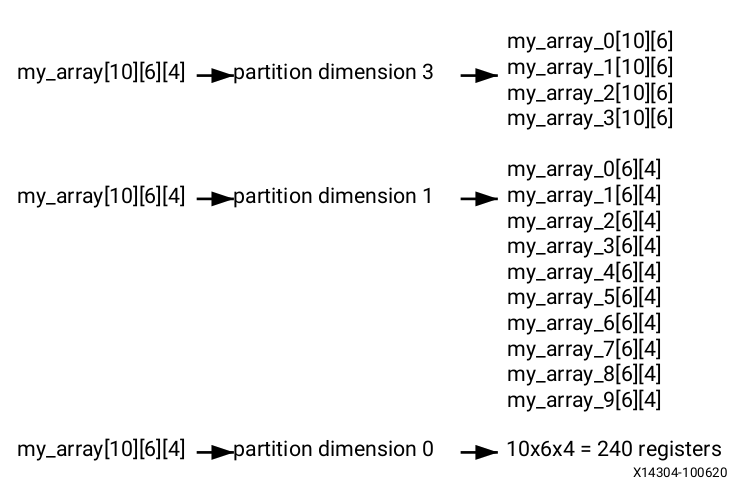
\includegraphics[scale=0.5]{images/float-partition-dim.png}
    \caption{Partitioning Array Dimensions}
    \label{fig:float-partition-dim}
\end{figure}

\begin{figure}[ht!]
    % \centering
    \begin{subfigure}[b]{\textwidth}
        \inputminted[firstline=3]{diff}{program/1c1-partition-ap-d1-f2.diff}
        \caption{Setting array partition with \texttt{dim}=1}
        \label{fig:1c1-partition-ap-d1-f2.diff}
    \end{subfigure}
    \begin{subfigure}[b]{\textwidth}
        \inputminted[firstline=3]{diff}{program/1c1-partition-ap-d2-f2.diff}
        \caption{Setting array partition with \texttt{dim}=2}
        \label{fig:1c1-partition-ap-d2-f2.diff}
    \end{subfigure}
    \caption{Comparing different setting of \texttt{dim}}\label{fig:1c1-partition-d12}
\end{figure}

I have also experimented on this, where the code is modified as \autoref{fig:1c1-partition-d12}.
The HLS summary (\autoref{tab:float-summary}) shows setting \texttt{dim} to 1, producing the same number of adders and multipliers, introduces more resource usage but the latency is worse.
On the contrary, setting \texttt{dim} to 2 leads to introducing more floating-point adders and multipliers and achieves a lower latency.
The result also supports our conclusion above.

%%%%%%%%%%%%%%%%%%%%%%%%%%%%%%%%%%%%%%%%%%%%%%%%%%%%%%%%%%%%%%%%%%%%%
\subsubsection{Trying different \texttt{factor}s}\label{sec:1cFac}

As shown in \autoref{tab:float-summary}, when \texttt{factor}=8, the latency is reduced to 4911, which means 46.4x improvement, where 16 floating-point adders and 16 floating-point multipliers are used.
When \texttt{factor}=16, the latency is reduced to 4279, which means 53.3x improvement, where 32 floating-point adders and 32 floating-point multipliers are used.
That is exactly 16 times of that when array partition is not used.
From \autoref{tab:float-loop-1c2-partition-ap-d2-f8} and \autoref{tab:float-loop-1c2-partition-ap-d2-f16}, it can be seen that the initiation interval is 16 cyles when \texttt{factor}=8 and 8 cycles when \texttt{factor}=16.
Adding the \texttt{factor} to 32 makes the utilization of DSP and LUT exceeds the resource budget.

\begin{table}[ht!]
    \caption{Loop details for partition with \texttt{dim}=2 \texttt{factor}=8}
    \label{tab:float-loop-1c2-partition-ap-d2-f8}
    \centering
    \begin{tabularx}{\textwidth}{ p{4cm} *{7}{C}}
    \toprule
    \multicolumn{1}{c}{\multirow{2}{*}{Loop Name}} &
    \multicolumn{2}{c}{Latency (cycles)}           &
    \multicolumn{1}{c}{\multirow{2}{*}{\makecell*{Iteration \\
    Latency}}}                                     &
    \multicolumn{2}{c}{Initiation Interval}        &
    \multicolumn{1}{c}{\multirow{2}{*}{\makecell*{Trip      \\
    Count}}}                                       &
    \multicolumn{1}{c}{\multirow{2}{*}{Pipelined}}          \\

    \cmidrule(lr){2-3}
    \cmidrule(lr){5-6}

                                                   &
    \multicolumn{1}{c}{min}                        &
    \multicolumn{1}{c}{max}                        &
                                                   &
    \multicolumn{1}{c}{achieved}                   &
    \multicolumn{1}{c}{target}                     &        \\
    \midrule
    \texttt{- LOAD\_OFF\_1} & 5 & 5 & 1 & 1 & 1 & 5 & yes \\
\texttt{- LOAD\_W\_1\_LOAD\_W\_2} & 1280 & 1280 & 1 & 1 & 1 & 1280 & yes \\
\texttt{- LOAD\_I\_1\_LOAD\_I\_2} & 1024 & 1024 & 1 & 1 & 1 & 1024 & yes \\
\texttt{- L1\_L2} & 2550 & 2550 & 1287 & 16 & 1 & 80 & yes \\
\texttt{- STORE\_O\_1\_STORE\_O\_2} & 42 & 42 & 4 & 1 & 1 & 40 & yes \\
    \bottomrule
\end{tabularx}

\end{table}

\begin{table}[ht!]
    \caption{Loop details for partition with \texttt{dim}=2 \texttt{factor}=16}
    \label{tab:float-loop-1c2-partition-ap-d2-f16}
    \centering
    \begin{tabularx}{\textwidth}{ p{4cm} *{7}{C}}
    \toprule
    \multicolumn{1}{c}{\multirow{2}{*}{Loop Name}} &
    \multicolumn{2}{c}{Latency (cycles)}           &
    \multicolumn{1}{c}{\multirow{2}{*}{\makecell*{Iteration \\
    Latency}}}                                     &
    \multicolumn{2}{c}{Initiation Interval}        &
    \multicolumn{1}{c}{\multirow{2}{*}{\makecell*{Trip      \\
    Count}}}                                       &
    \multicolumn{1}{c}{\multirow{2}{*}{Pipelined}}          \\

    \cmidrule(lr){2-3}
    \cmidrule(lr){5-6}

                                                   &
    \multicolumn{1}{c}{min}                        &
    \multicolumn{1}{c}{max}                        &
                                                   &
    \multicolumn{1}{c}{achieved}                   &
    \multicolumn{1}{c}{target}                     &        \\
    \midrule
    \texttt{- LOAD\_OFF\_1} & 5 & 5 & 1 & 1 & 1 & 5 & yes \\
\texttt{- LOAD\_W\_1\_LOAD\_W\_2} & 1280 & 1280 & 1 & 1 & 1 & 1280 & yes \\
\texttt{- LOAD\_I\_1\_LOAD\_I\_2} & 1024 & 1024 & 1 & 1 & 1 & 1024 & yes \\
\texttt{- L1\_L2} & 1918 & 1918 & 1287 & 8 & 1 & 80 & yes \\
\texttt{- STORE\_O\_1\_STORE\_O\_2} & 42 & 42 & 4 & 1 & 1 & 40 & yes \\
    \bottomrule
\end{tabularx}

\end{table}

% %%%%%%%%%%%%%%%%%%%%%%%%%%%%%%%%%%%%%%%%%%%%%%%%%%%%%%%%%%%%%%%%%%%%%
\subsection{Amortizing Iteration Latency with Batching (8 marks)}
%%%%%%%%%%%%%%%%%%%%%%%%%%%%%%%%%%%%%%%%%%%%%%%%%%%%%%%%%%%%%%%%%%%%%

Report \begin{enumerate}
    \item the design latency in cycles, and
    \item the overall device utilization (as Total per Resource).
\end{enumerate}


%%%%%%%%%%%%%%%%%%%%%%%%%%%%%%%%%%%%%%%%%%%%%%%%%%%%%%%%%%%%%%%%%%%%%

\section{Part 2: Fixed-Point Optimizations (30 marks)}

\begin{enumerate}
  \item the fixed-point validation accuracy reported by mnist.py after you've tweaked the SCALE factor.
  \item the design latency in cycles
  \item the overall device utilization (as Total per Resource).
  \item your measured system speedup over the fixed-point CPU implementation
  \item your measured classification accuracy on the 8k MNIST test sample
  \item how many multipliers are instantiated in your desing?
  \item report the initiation interval of the matrix multiplication loop that you pipelined
  \item given the number of multipliers in your design and input throughput via the AXI port, is the design bandwidth- or compute-limited?
\end{enumerate}

\section{Part 3: Open-ended design optimization (30 marks)}

\href{https://www.xilinx.com/support/documentation/sw_manuals/xilinx2020_2/ug1399-vitis-hls.pdf}{Vitis High-Level Synthesis User Guide}


% \bibliographystyle{ACM-Reference-Format}
% \bibliography{base}

\clearpage
\appendix

\end{document}
\endinput
